\chapter{Test}
This chapter focus on testing the game in two ways. First there is a user test which seeks to find to which extent the game fits the target group. Secondly there is a test which focus on the performance on the game.

\section{User test}
The main goal of the game is to cater for hardcore players, the relevant factors in order to do this are outlined in table \ref{tab:gamerdedication}.
The purpose of the test is to discover to which extent the game caters to hardcore players.
This will be done by creating a test which will take the players through the games features which show off all factors which cater \emph{hardcore} gamers, described in Section \ref{gamedesign:selectionofgametype}.
This means the player should:
\begin{itemize}
	\item Experience leveling your character
	\item Experience crafting weapons/upgrades
	\item Experience an objective
	\item Kill some aliens
	\item Playing with multiple classes on the team
\end{itemize}

The player will however, not try to create their own mission packs. The main reason for this is that the data-format of the custom content is JSON and rather large. It would take a considerable amount of time to get familiar with the syntax and formatting of this file, which is not doable. More on this is described in \tododennis{Insert todonote for discussion}.

\section{User Profile}
The users intended for this test are hardcore players.
To find test subjects within this segment, a preliminary survey has been made to determine whether or not the player is hardcore.
The survey will more specifically determine the players \textit{Gamer Dedication Score} which is based on the Gamasutra article\cite{casual_vs_hardcore} outlined in motivation, Section \ref{sec:motivation}.
All the factors from the article have been turned into questions, as even the ones we cannot affect during game design are relevant to classify players.
For each question, 5 answers exist ranging from \textit{"I strongly disagree"} to \textit{"I strongly agree"}.

The answers are then used to evaluate Equation \ref{eq:GD} in order to determine a \emph{gamer dedication score}.
The goal is to find a group of \emph{hardcore} players or \emph{ultra hardcore} players to use for the test.
The full survey and the complete results can be found in Appendix \ref{app:survey}.

\section{Context, Equipment \& Setup}
The test will take place in one of the group rooms of Cassiopeia at Aalborg University.
Each team will consist of three to four players.
The players will be equipped with three mobile devices and a computer.

\subsection{Mission}
The game will be played with a premade mission pack that is designed to show a realistic game session in the completed game.
The mission pack consists of two missions.
The first contains two waves - Each wave will introduce a new enemy each wave.
Following that, the second mission contains three waves - The first two will introduce new enemies and the last wave will introduce a boss.
The mission should furthermore enable all the players to get enough resources to try out different weapons and their upgrades.

\section{Tasks}
To show the players the features the following tasks should be done:
\begin{enumerate}
	\item Players starts by joining a game lobby together
	\item Player then should select their favoured class
	\item The host will select the mission created for the purpose
	\item The players should then attempt to complete the mission pack
\end{enumerate}
If the team should fail the mission pack, they should try again but have time to discuss strategy.

\section{Post-play questionnaire \& results}\label{test:results}
A post-game survey is taken by the test subjects in order to determine to which extent they enjoy the concepts that have been designed to facilitate the gameplay catering to hardcore players.
The purpose is to determine if the game adequately satisfies the goals set up in Section \ref{sec:motivation} and the problem statement in Section \ref{sec:specifyingtheproblemstatemen}.
The full questionnaire and results can be found in the Appendix, Section \ref{app:postgame}.
A summary of the are as follows:
\begin{enumerate}\label{test:post-play}
\item \textbf{What did you think of the concept of waves in the game?}\vspace{4pt}\\
The general response was that the test subjects liked the concept.
One player expressed that he would have preferred a constant assault instead of the wave system.

\item \textbf{What did you think of the concept of objectives which yield rewards?}\vspace{4pt}\\
The general response was that the test subjects did not know of or understand the objective system.
Some players confused the objective system with the loot system.

\item \textbf{What did you think of the concept of player classes and traits?}\vspace{4pt}\\
The test subjects generally agreed that it added complexity and strategy to the game, but it was not easy to see the difference between the different classes.

\item \textbf{What did you think of the weapons and their upgrades?}\vspace{4pt}\\
Two test subjects mentioned that controlling shooting on a mobile device is impossible due to the aiming and shooting controls being linked.
Four test subjects were not able to try weapons and upgrades due to not noticing the feature.
One subject expressed that he would like to be able to trade resources with other players.
Half of the test subjects liked the system.

\item \textbf{What did you think of the overall difficulty of the game?}\vspace{4pt}\\
There were two general responses.
Half of the test subjects liked the difficulty, the other half thought it was a bit too hard.
One player mentioned that he liked that the game was difficult because he thinks there are too many casual games today.

\item \textbf{Did you find a single game session long enough to entertain you?}\vspace{4pt}\\
Most subjects found that the single game session was long enough to entertain them, only one test subject wanted a longer session.

\item \textbf{Did you find the game frustrating at times?}\vspace{4pt}\\
The test subjects largely agreed that the control scheme for touch-devices was frustrating, mainly due to not being able to aim without shooting.
One subject found that the he was frustrated when the game crashed.

\item \textbf{Would you consider modifying the game with additional maps and missions, if tools were supplied for doing so?}\vspace{4pt}\\
Half of the subjects would consider creating additional maps and missions.

\item \textbf{Did you find satisfaction in completing the game?}\vspace{4pt}\\
Most of the test subjects felt satisfaction upon completing waves.
The only test subject that managed to beat the boss and the final wave expressed that he was not aware that he had won, due to the short line of sight.

\item \textbf{Did you find yourself engaged in competition with yourself, the enemies or other players while playing the game?}\vspace{4pt}\\
All the test subjects agreed that that they were engaged in competition with each other.
One subject wrote that he actually was more competitive about the lootable resources, than the score.

\item \textbf{Did you find the game having potential to be deep and complex, if more content was added?}\vspace{4pt}\\
Most of the test subjects thought the game had potential to be deep and complex if more content was added.
Some of the test subjects thought that there was already too many traits.

\item \textbf{Would you classify the game as an action game?}\vspace{4pt}\\
All except one test subject answered that they thought the game is an action game.
The one that didn't explained that it is because action games requires one to react to changes quickly, and he did not feel our game required this of him.

\item \textbf{Did you find the game fun?}\vspace{4pt}\\
All the test subjects agreed that the game was fun.
\end{enumerate}

\section{Result Analysis}
Overall the test subjects were largely happy about the gameplay and content designed to cater to hardcore gamers.
From this we gather that designing a game based on the factors mentioned in Table \ref{tab:relevantFactors} enables the game to cater to hardcore players as defined by Gamasutra\cite{casual_vs_hardcore}.

\section{Performance test}
The goal of the performance test is to figure out whether or not the framerate in the game is acceptable according to requirement 8 in section \ref{gamedesign:selectionofgametype:importantstuff}. 

\subsection{Setup}
Multiple tests will be run, but it is important to keep variables constant to focus on specific parts of the test. In order to do this the same wave of the same mission will be tested everytime. The test session will last until the wave has been completed. 

The test will be done with multiple setups:
\begin{itemize}
\item Performance test on PC and Mobile while playing alone
\item Performance test of the server in a two player game, both mobile and pc platform
\item Performance test of the server when it deals with a higher number of players
\end{itemize}

The reason the game is tested in solo mode, is to create a baseline for both platforms. That is, how fast and smooth does the game run if you are the only client, and the only server. In this scenario, the server will not handle other input but its self.

The second scenario is running it with another player. This is done to see how the game, and server in particular, handles multiple game clients. This is interesting because the server handles all logic in the game, and basically instructs the clients to do ''its bidding''. So the more clients, the more the server has to do. 

The last test is to see how it scales to a full game which is 3-4 players. It is interesting because not only does the amount of objects in the game increase vastly, e.g. bullets, but it also means the network traffic increases and the server load increases. Does it scale linearly or are there significant drops as more clients connect?

\subsection{Results}
\subsection*{Server performance}
The main goal for having an acceptable FPS is that it is relatively high and more importantly smooth without dips. Figure \ref{test:performance:pcserverone} and figure \ref{test:performance:mobileserverone} shows the performance of a single player who is also the server, on PC and mobile respectively. Although the PC runs 150 frames per second more than the mobile server, they both share the same characteristics that the server runs extremely smoothly. The PC has an average fps of \emph{195} where the mobile has an average of \emph{57}. Both of these values are well above our goal of \emph{60} fps and \emph{45} fps for PC and mobile respectively. Additionally if you look at the data, there is a large drop in FPS at the very beginning of each data-set. This drops goes for a few frames with a few players and a few more frames if there is 4 players or more. These frames are when the server and clients load all data, so they are to be expected and have no real impact on the game flow. The actual numbers for the different tests for a server can be seen summed up in table \ref{test:table:data}. The complete data sets can be seen in Appendix \ref{appendix:test:fpsdata}.
\begin{figure}
    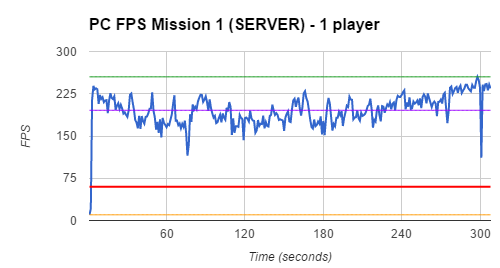
\includegraphics{figures/test/PCServerOnePlayer}
    \caption{PC server with one player (no clients) \\ Legend: Blue: FPS, Purple: Average FPS, Green: Max FPS, Yellow: Minimum FPS, Red: Target FPS}
    \label{test:performance:pcserverone}
\end{figure}

\begin{figure}
    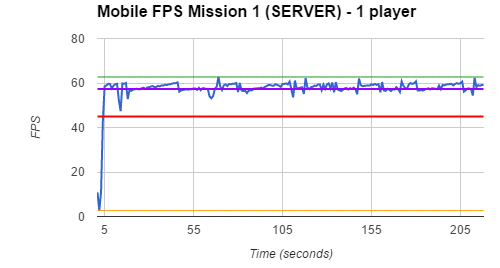
\includegraphics{figures/test/MobileServerOnePlayer}
    \caption{Mobile server with one player (no clients) \\ Legend: Blue: FPS, Purple: Average FPS, Green: Max FPS, Yellow: Minimum FPS, Red: Target FPS}
    \label{test:performance:mobileserverone}
\end{figure}

\begin{table}[h]
\begin{tabular}{lllll}\label{test:table:data}
Platform/Game Clients & Average FPS & Minimum FPS & Maximum FPS &  \\
PC / 1 player         & 195         & 10          & 255         &  \\
PC / 2 player         & 247         & 10          & 266         &  \\
PC / 3 player         & 220         & 9           & 256         &  \\
Mobile / 1 Player     & 57          & 3           & 62          &  \\
Mobile / 2 Player     & 56          & 3           & 63          &  \\
Mobile / 3 Player     & 57          & 3           &             & 
\end{tabular}
\caption{The average, minimum and maximum FPS for the server in different test results (data is rounded) }
\end{table}

One thing to note is the fact that the PC server will fluctuate 10-30%  in FPS, where as the mobile normally fluctuates between 0-10% and rarely 20%. This happens mostly if there is 3 or more players connected, but it still keep a running minimum fps well above the minimum fps we set as a target though and one could easily cap the server to 120FPS to keep a rock steady frame rate.

\subsection*{Client performance}
The client performance is much equal to the server. A PC will run roughly \emph{250} and the mobile will run in the area of \emph{55} fps. A graph for a PC connected to a mobile server can be seen in \ref{test:performance:pcclientmobileserver} and a graph for a mobile client can be seen in figure \ref{test:performance:mobileclientpcserver}.

\begin{figure}
    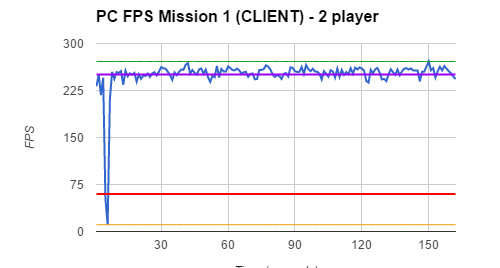
\includegraphics{figures/test/PCClient2Player}
    \caption{PC client connected to a mobile server \\ Legend: Blue: FPS, Purple: Average FPS, Green: Max FPS, Yellow: Minimum FPS, Red: Target FPS}
    \label{test:performance:pcclientmobileserver}
\end{figure}

\begin{figure}
    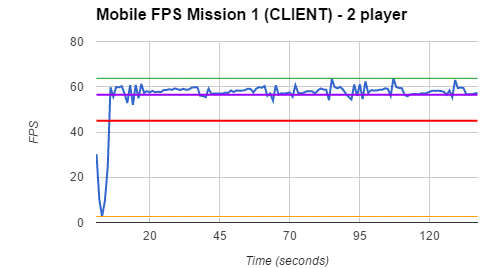
\includegraphics{figures/test/MobileClient2Player}
    \caption{Mobile client connected to a pc server \\ Legend: Blue: FPS, Purple: Average FPS, Green: Max FPS, Yellow: Minimum FPS, Red: Target FPS}
    \label{test:performance:mobileclientpcserver}
\end{figure}

